% The MIT License (MIT)
%
% Copyright (c) 2020 Yegor Bugayenko
%
% Permission is hereby granted, free of charge, to any person obtaining a copy
% of this software and associated documentation files (the "Software"), to deal
% in the Software without restriction, including without limitation the rights
% to use, copy, modify, merge, publish, distribute, sublicense, and/or sell
% copies of the Software, and to permit persons to whom the Software is
% furnished to do so, subject to the following conditions:
%
% The above copyright notice and this permission notice shall be included
% in all copies or substantial portions of the Software.
%
% THE SOFTWARE IS PROVIDED "AS IS", WITHOUT WARRANTY OF ANY KIND, EXPRESS OR
% IMPLIED, INCLUDING BUT NOT LIMITED TO THE WARRANTIES OF MERCHANTABILITY,
% FITNESS FOR A PARTICULAR PURPOSE AND NON-INFRINGEMENT. IN NO EVENT SHALL THE
% AUTHORS OR COPYRIGHT HOLDERS BE LIABLE FOR ANY CLAIM, DAMAGES OR OTHER
% LIABILITY, WHETHER IN AN ACTION OF CONTRACT, TORT OR OTHERWISE, ARISING FROM,
% OUT OF OR IN CONNECTION WITH THE SOFTWARE OR THE USE OR OTHER DEALINGS IN THE
% SOFTWARE.

\documentclass[sigplan,10pt,screen]{acmart}
% \settopmatter{printfolios=false,printccs=false,printacmref=false}

\title{Volatility Metric to Detect Anomalies in Source Code Repositories}
\author{Yegor Bugayenko}
\orcid{0000-0001-6370-0678}
\email{yegor256@gmail.com}
\affiliation{\institution{}\city{Moscow}\country{Russia}}

\setcopyright{acmcopyright}
\acmPrice{15.00}
\acmDOI{10.1145/3486949.3486961}
\acmYear{2021}
\copyrightyear{2021}
\acmSubmissionID{splashws21bcncmain-p41-p}
\acmISBN{978-1-4503-9125-2/21/10}
\acmConference[BCNC '21]{Proceedings of the 1st ACM SIGPLAN International Workshop on Beyond Code: No Code}{October 17, 2021}{Chicago, IL, USA}
\acmBooktitle{Proceedings of the 1st ACM SIGPLAN International Workshop on Beyond Code: No Code (BCNC '21), October 17, 2021, Chicago, IL, USA}

\begin{CCSXML}
<ccs2012>
<concept>
<concept_id>10011007.10011074.10011111.10011696</concept_id>
<concept_desc>Software and its engineering~Maintaining software</concept_desc>
<concept_significance>500</concept_significance>
</concept>
</ccs2012>
\end{CCSXML}
\ccsdesc[500]{Software and its engineering~Maintaining software}
\keywords{Metrics, Software Size, Software Maintainability}

\usepackage[utf8]{inputenc}
\usepackage{textcomp}
\usepackage[inline]{enumitem}
\usepackage{amsmath}
\usepackage{graphicx}
\usepackage{pgfplots}
\usepackage{verbatimbox}
\usepackage{interval}
\usepackage{hyperref}
\usepackage{minted}
  \setminted{fontsize=\footnotesize}
  \setminted{breaklines}
  \usemintedstyle{bw}
\newcommand{\code}[1]{\texttt{#1}}
\newenvironment{nicetable}
  {\setlength{\parindent}{0em}\medskip\small}
  {\medskip}
\def\thetotaljavafiles{10023}
\def\thetotalrepos{240}

\begin{document}
\begin{abstract}
A new metric was introduced to calculate the distance
between actively modified files in a source code repository
and the files, which are rarely modified and may be considered
abandoned or even dead. It was empirically demonstrated that larger repositories
have larger values of the introduced metric.
The metric may be used for earlier detection of code maintenance anomalies
and helping software developers make the decision of splitting the repository
into smaller ones in order to prevent maintainability issues.
\end{abstract}
\maketitle

\section{Introduction}

Most software development projects keep their source code in Git~\citep{loeliger2012},
which is the de-facto standard in the industry at the moment, or similar
version control systems. Every system, including open
source products like Git, Subversion, and Mercurial, and commercical tools
like StarTeam\texttrademark{} or ClearCase\texttrademark{}
have the same feature: keeping track of the changes
made to the source code files, also known as ``logs.''

Git logs provide information about every single change made by every software
developer during the entire course of the project. Using this information
it's possible to measure which files are being modified more frequently than others.
On the other hand, it's also possible to spot files that are rarely modified and may
be considered either as \emph{abandoned} or \emph{stable} code.
\citet{fontana2014} claims that the gap between actively modified code
and the code that is stable should be as narrow as possible in a properly
maintained repository.

Indeed, abandoned code may be considered as a threat
to the maintainability of the entire project, because its lifecycle
is not aligned with the lifecycle of active code, which is modified more intensively.
Later, when a modification is required to the abandonded code, a programmer
may have difficulties finding out the principles of design of the code and
making sure new modifications don't break it.

We introduce a Volatility metric to measure the relationship
between the amount of actively modified files and files which stay
in the repository for a long time without modifications.
The hipothesis is that the Volatility is related to the size of the
repository: the larger the repository the higher the volatility. Larger
repositories are an obvious threat to code maintainability. Thus, if
the relationship between size and Volatility exists, the new metric
can be used to identify code anomalies and detect badly maintained repositories.

In order to validate the hipothesis and demonstrate how the metric works we applied it to
\thetotalrepos{} public Java repositories from GitHub and analyzed
its impact on two other characteristics of each repository:
the number of files in a repository and the size of it in bytes.

Larger repositories shown larger values of the metric.

The paper is organized as follows.
Section~\ref{sec:background} defines various terms used in the paper.
Section~\ref{sec:related} covers related work in the areas of code change metrics
and empirical analysis of source code repository size.
Section~\ref{sec:method} covers the source code volatility metric.
Section~\ref{sec:results} covers our empirical case study of \thetotalrepos{} Java source code repositories.
Section~\ref{sec:discussion} covers limitations of both the metric and the study.
Finally, we summarize our study in Section~\ref{sec:conclusion}.

\section{Background}
\label{sec:background}

In this paper, we use several terms regarding version control systems and
software metrics. The type of metric we are proposing belongs to the family
of \emph{source code change metrics}, which analyze the history
of changes in a source code repository~\citep{fentonsoftware,choudhary2018}.
A \emph{change} in a version control system, such as Git, is an atomic
modification to the source code file made by a software developer locally
on his/her machine and then \emph{committed} to the repository.

Each version control system, including Git, provides an instrument for
retrieving the entire history of changes from a repository. We use
\texttt{git log} for Git.

GitHub\texttrademark{} (currently owned by Microsoft\texttrademark{}) is
one of the largest platforms for \emph{open source} projects.
GitHub provides free access to all public Git repositories, which makes it possible
to analyze Git histories.

\section{Related Work}
\label{sec:related}

``Code change metrics mined from source control repositories have
proven to be the most reliable predictors of bugs in
contemporary software engineering research,'' says \citet{muthukumaran2015}.

Code churn is one of the simplest metric in the family, which counts
all lines being modified (added, edited, and deleted) during
the entire lifetime of a project~\citep{munson1998}. It was demonstrated
by~\citet{shin2010} how code churn, together with complexity and other
developer activity metrics, is related to software vulnerabilities. There
are modifications of code churn, for example taking into accout socio-technical
aspect of the metric, as suggested by~\citet{meneely2012}.

Yet another simple metric from the family is
the number of changes being made to a particular file, class, method
or line of code, which is used for example by~\citet{demeyer2000}
in order to analyze the effect of refactorings.

\citet{moser2008} made a comparative analysis of 17 change metrics to understand
their efficiency for defect prediction: number of distinct authors per file,
total modifications per file, total additions per file, maximum number of
files committed together, and others.

\citet{biazzini2014} introduced a number of metrics to analyze
Git history (specifically related to GitHub), such as unique-count, unique-ratio,
VIP-count, VIP-ratio, scattered-count, pervasive-count and a few others. Some
of the metrics are supposed to be calculated for a repository together with
its forks, while others may be calculated for a single repository history.

\citet{batista2018} provided a detailed analysis of existing metrics
and introduced a new one to measure, by looking at Git/GitHub project
commit history, how ``close'' developers stay to each other and form
pairs.

\citet{fontana2014} suggested to measure ``File Volatility'' as the ratio
between the maximum number of changes happened to a file line and the number
of all changes to the file since its creation. Going further, they also suggested to
calculate ``Repository Stability'' metric as a relationship between
active files (with high File Volatility) and closed files.
The also concluded that repositories where most files change
over time can suffer from organizational or design issues.

To our knowledge, the metric introduced in this research, in order
to detect anomalies in source code repository maintenance, has never been
suggested.

\section{Metric}
\label{sec:method}

First, by looking at the Git history,
it is observed how many times every source code file out of $N$ was touched
during the lifetime of the repository (excluding the files that don't exist
in the repository anymore):

\begin{eqnarray}
T = [t_1, t_2, \dots, t_N]
\end{eqnarray}

Here, $t_i$ is the number of commits found in the repository, which
modified the $i$-th file. Then, the entire interval between $\check{T}$ (the maximum value)
and $\hat{T}$ (the minimum value) is divided to $Z$ (the input parameter of the method)
equivalent groups:

\begin{align}
\delta &= ( \check{T} - \hat{T} ) / Z \\
G &= [g_1, g_2, \dots, g_{Z}] \\
g_j &= \sum_{i=1}^N [ j \times (\delta-1) < t_i < j \times \delta ]
\end{align}

Here, $g_j$ is the total number of $t_i$, which are larger than
$j \times (\delta-1)$ and smaller than $j \times \delta$. In other words,
$T$, the entire set of measurements, is sorted and then split into $Z$ sectors,
where $g_j$ is the counter of measurements that belong to the sector $j$.

Then, the mean $\mu$ is calculated as:

\begin{eqnarray}
\mu = \frac{1}{Z}\sum_{j=1}^{Z}{g_j}
\end{eqnarray}

Finally, the variance is calculated as:

\begin{eqnarray}
\text{Var}(g) = \frac{1}{Z}\sum_{j=1}^{Z}{|g_j - \mu|^2}
\end{eqnarray}

The variance $\text{Var}(g)$ is the Volatility of the source code. The smaller
the Volatility the more cohesive is the repository and the smaller
the amount of the abandonded code inside it. The metric demonstrates how
large is the gap between intensively modified files and the abandoned ones:
the larger the variance, the wider the graph, and the larger the gap.
A repository with a thousand files all being modified at the same pace would
have a Volatility of zero. On the other hand, a repository with just a few
files, where one of them is modified a thousand times, while others are modified
just once, will have the Volatility of a miillion.

\section{Empirical Results}
\label{sec:results}

A list of Java repositories were retrieved from GitHub via their
public API. The first \thetotalrepos{} repositories were taken, which satisfied
the selection criteria:
\begin{enumerate*}[label={\arabic*)}]
\item more than 1,000 GitHub stars,
\item more than 200 Kb of data,
\item not archived, and
\item public.
\end{enumerate*}
The list included popular Java open source products, such as
Spring, RxJava, Guava, MyBatis, Clojure, JUnit, Lombok,
Graal, Selenium, Spark, Mockito, Neo4j, Jenkins, Netty, and others.

The Volatility metric was calculated for each repository, using the
formula explained above (the value of $Z$ was set to 64).
Then, a few other metrics were collected
for each repository and their values were compared with the Volatility.

The Figure~\ref{fig:1} demonstrates the relationship between
the number of files in the repository~($M_1$) and its Volatility~($V$).
Both axixes of the graph have logarithmic scales, for the sake of visual
understandability: the difference between the minimum and the maximum values
of the Volatility is logarithmically large. It is visually obvious that
repositories with larger number of files tend to have higher values
of the Volatility metric.

\begin{figure}[h]
  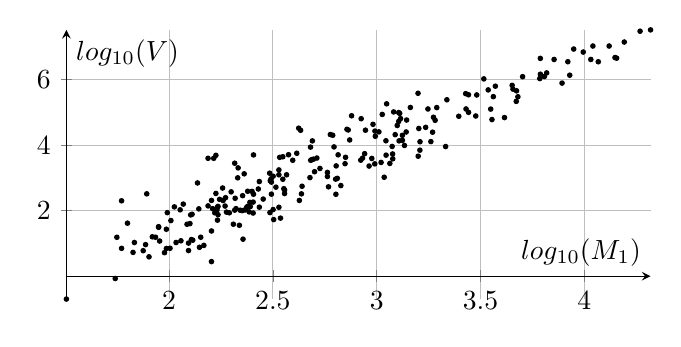
\begin{tikzpicture}
\begin{axis}[width=9cm,height=5cm,
axis lines=middle, xlabel={$log_{10}(M_1)$}, ylabel={$log_{10}(V)$},
xmin=1.5051499783199058, xmax=4.319480828050337,
ymin=-0.6989700043360187, ymax=7.518906770153717,
extra tick style={major grid style=black},grid=major]
\addplot [mark=*, only marks, mark size=0.8pt] coordinates {
(2.110589710299249,1.8893017025063101)
(2.02530586526477,2.1161648123118737)
(2.2253092817258624,3.690196080028514)
(1.919078092376074,1.2024201977780304)
(2.3783979009481375,2.132259689531044)
(1.9493900066449126,1.5114377022035417)
(2.5563025007672873,2.6290590146121775)
(3.8930401119571174,5.894521592313384)
(2.827369273053825,2.766366366191725)
(2.2041199826559246,2.313041477993241)
(2.810232517995084,2.986221321921366)
(2.945960703577568,4.456556889858923)
(2.53655844257153,1.7723217067229198)
(2.9319661147281724,3.603570810833047)
(2.3304137733491905,3.0024017071695166)
(3.048053173115609,5.261700987694412)
(2.681241237375587,3.9397355140239028)
(2.624282095835668,4.516641125276831)
(2.762678563727436,3.043885997687633)
(2.187520720836463,3.598681098907163)
(3.9301336458411176,6.135328024033434)
(3.8189513116401725,6.205079897573985)
(1.9867717342662448,1.4326486600131065)
(2.3096301674258983,1.5861651813773168)
(2.187520720836463,2.1455071714096623)
(2.0530784434834195,2.0255984179691437)
(2.3617278360175926,3.1246296093882875)
(3.949194774237982,6.933645525949034)
(2.9934362304976116,4.270899536716091)
(2.850033257689769,3.62935862258034)
(2.2095150145426303,2.060225524394167)
(3.9951962915971793,6.842255669870494)
(2.4533183400470375,2.353723937588949)
(3.077367905284156,3.5823056337991357)
(2.4065401804339546,3.7015679850559273)
(2.086359830674748,1.5846542400042958)
(2.2329961103921536,2.110910222862586)
(3.208710019906401,4.104214833202107)
(1.7993405494535815,1.6174663223227894)
(3.1338581252033344,3.991060867336677)
(3.4426365257822313,5.0012477132165465)
(3.2692793897718984,4.3953798183655985)
(4.2689989585426735,7.4785919782652845)
(2.5289167002776547,3.2433253064048313)
(3.332236415491443,3.957451640973415)
(2.2304489213782737,2.021348352175276)
(3.2030328870147105,4.508943616417986)
(3.010723865391773,4.404937193444941)
(2.633468455579586,4.453807410461225)
(2.4857214264815797,1.9413544870741446)
(1.9542425094393248,1.0725506672154261)
(3.2736955879300917,4.850314498869368)
(3.0362295440862943,3.0197451611626906)
(2.5327543789924976,3.6285539698935225)
(2.8627275283179743,4.46364463341919)
(2.3541084391474008,2.4576490310602934)
(2.804820678721162,3.3661253696265216)
(2.2430380486862944,2.3463529744506384)
(2.7767011839884104,4.324195541965875)
(2.4345689040341987,2.10744390151416)
(3.5162708827293403,6.02280213455429)
(2.3384564936046046,1.5531981666918748)
(2.404833716619938,1.9276674643013594)
(2.487138375477186,2.9149510611278813)
(2.869818207979328,4.158550947069742)
(3.261024833992397,4.108868594335923)
(3.021189299069938,3.473347917960341)
(3.2469906992415494,5.1043407000326795)
(2.3521825181113623,2.0012553521371235)
(4.120014252078067,7.026345332117251)
(1.7708520116421442,2.301029995663981)
(2.3180633349627615,2.3781070625097422)
(2.3729120029701067,2.094988884153331)
(1.8750612633916997,0.7781512503836435)
(2.5289167002776547,3.0950995796456136)
(2.700703717145019,3.1888972496655783)
(3.442322955745574,5.538261383647847)
(2.81424759573192,3.7043333313349556)
(3.703033304733686,6.0899937855546495)
(3.1442627737619904,4.766828386772239)
(2.925312091499649,4.807671991878399)
(3.7884512070234555,6.648699032636881)
(3.854731017213942,6.61545105201613)
(3.162265614298021,5.150568494793861)
(3.1149444157125843,4.8112124638026295)
(2.726727209026572,3.288966121430523)
(4.031650793551264,6.615811349712656)
(1.7708520116421442,0.8495071588315756)
(2.3159703454569174,2.0160241898425677)
(3.0633333589517493,3.4416390361140126)
(2.2355284469075487,2.1285204277315373)
(2.8020892578817325,2.962759882966592)
(2.404833716619938,2.26150077319828)
(1.5051499783199058,-0.6989700043360187)
(2.6148972160331345,3.7516126536562173)
(2.7118072290411908,3.6070754167873944)
(2.963315511386111,3.361809651907951)
(2.093421685162235,0.7820462939763456)
(3.3382572302462554,5.385552504732252)
(3.5493711523331766,5.1009217642820515)
(2.3856062735983117,1.9619979741284004)
(2.923244018630276,3.5410172928456563)
(3.123851640967086,4.299841039569371)
(1.9867717342662448,0.8450980400142567)
(2.008600171761917,1.6983905586147934)
(2.847572659142112,3.434283999039787)
(2.2041199826559246,0.4447181689885548)
(3.20002926655377,3.662411516877962)
(2.1003705451175625,1.6055205234374688)
(2.8567288903828825,4.484465931154977)
(2.803457115648414,2.4999209514943916)
(3.4820155764507117,5.53258298931776)
(2.9916690073799486,4.4295863158722355)
(2.678518379040114,3.0093528203388042)
(3.106190897263415,4.995030190801473)
(3.6737579365495763,5.6591937624128725)
(2.2329961103921536,1.7101173651118162)
(3.6526330680831096,5.826252697358896)
(3.098989639401177,4.6003901802505185)
(2.2988530764097064,2.5740922170633866)
(3.4772659954248524,4.890209444341324)
(3.785756799962643,6.033105739540872)
(2.976349979003273,3.5942733022270197)
(1.8920946026904801,2.513550520346337)
(1.9777236052888476,0.7174534096681198)
(2.2253092817258624,2.5255306856799953)
(2.0681858617461617,2.200224938768488)
(3.106190897263415,4.724916108623423)
(4.319480828050337,7.518906770153717)
(3.788663213120857,6.165561437169954)
(2.4913616938342726,2.9721756022004318)
(3.1078880251827985,4.130724228165944)
(4.04166896647561,7.025922150535285)
(1.7481880270062005,1.187520720836463)
(2.214843848047698,3.5977682933213706)
(3.026941627959029,4.938002817389457)
(3.6565772913961134,5.710334473753581)
(2.2576785748691846,2.691544559996647)
(1.7403626894942439,-0.07058107428570727)
(2.4297522800024076,2.6621416653736167)
(2.5477747053878224,2.9588197569614003)
(2.6821450763738315,3.5387155892481412)
(2.501059262217751,2.0328319929325596)
(2.6901960800285134,4.130709994038458)
(2.5658478186735176,3.0954770343927818)
(2.695481676490197,3.5716942774601916)
(2.2695129442179165,2.140972339302524)
(3.5373152731120094,5.686215711535072)
(3.428782511496954,5.57203525029253)
(4.192957529884656,7.148177996370741)
(2.5477747053878224,3.6462185097533273)
(2.575187844927661,3.7078425891424036)
(2.093421685162235,1.0104027602969754)
(3.3955011243056257,4.880803796054198)
(2.4065401804339546,2.5019923596491322)
(2.7944880466591693,3.945860088342011)
(3.920957705955449,6.546939748123799)
(2.5563025007672873,2.5234342867464368)
(2.6374897295125104,2.5131815933913293)
(3.236033147117636,4.542896746285134)
(2.5526682161121927,2.6705440298657708)
(2.3654879848908994,2.020692678682028)
(3.1992064791616572,5.58324163433773)
(2.143014800254095,2.054883306283622)
(3.11092624226642,4.969853048925632)
(2.2355284469075487,1.877946951629188)
(2.7678976160180904,2.728353782021228)
(3.680335513414563,5.476289871258936)
(2.7881683711411673,4.3025985161739335)
(2.3560258571931225,1.1298988216695378)
(2.8790958795000723,4.897401639443342)
(2.390935107103379,2.1242433089466486)
(1.9912260756924949,1.9390197764486663)
(1.9493900066449126,1.4913616938342726)
(2.501059262217751,3.0505437913005267)
(2.9907826918031377,3.4286507867872538)
(2.1367205671564067,2.8459932798852767)
(2.271841606536499,2.394951732105887)
(2.342422680822206,2.0141438111386196)
(2.1673173347481756,0.9395192526186184)
(2.2600713879850747,2.3105547887740983)
(2.220108088040055,1.9349791314294458)
(1.8325089127062362,1.0280287237359604)
(3.2893659515200313,5.146962281374943)
(3.123851640967086,4.146913191718257)
(2.0043213737826426,0.8512583487190752)
(2.6404814369704215,2.744727494900168)
(2.503790683057181,1.7278331076343305)
(3.0445397603924107,4.133830565731892)
(1.8260748027008262,0.7257631810724322)
(2.9420080530223127,3.739466856356103)
(3.571825249040829,5.800150006002939)
(2.6884198220027105,3.5599963460325896)
(2.5954962218255737,3.5386545102378473)
(2.1461280356782377,0.881691842553922)
(3.0891983668051486,4.321050058646378)
(3.045322978786657,3.69469731223624)
(1.9030899869919433,0.5906804451232659)
(2.3996737214810375,2.588247341812548)
(2.6273658565927325,2.3120715213029315)
(3.074450718954591,3.960485047655226)
(2.107209969647868,1.1179739564353584)
(2.3783979009481375,2.59193522773433)
(4.06774020292624,6.5461988792249155)
(2.1139433523068365,1.0988359341978273)
(2.3891660843645326,2.254427221540668)
(1.9344984512435675,1.189056236092315)
(2.4345689040341987,2.8893311951884435)
(2.514547752660286,2.717080782383067)
(2.276461804173244,1.9551754732533502)
(1.8864907251724818,0.9631973520922511)
(2.484299839346786,3.1436587344094393)
(2.322219294733919,2.062525008876046)
(2.0569048513364723,1.0804274291099996)
(2.2041199826559246,1.3795644887491045)
(2.5289167002776547,2.103251815334661)
(3.2081725266671213,3.846428754772363)
(2.332438459915605,3.305474207654434)
(2.0334237554869494,1.0280287237359604)
(4.148263229636878,6.6743104750179905)
(3.1420764610732843,4.402329459586968)
(3.672467313068082,5.336247054846863)
(3.555457217204649,4.781308249662078)
(4.156094630639427,6.655799142923314)
(3.807805532270624,6.093707734963201)
(3.6158448828747014,4.8417115785119)
(3.430558769522757,5.104286217017372)
(3.0766404436703416,3.7308460003706565)
(2.492760389026837,2.871602121022312)
(3.562054829656378,5.48085802900349)
(2.290034611362518,1.9343498983389538)
(3.081707270097349,5.014215921798604)
(2.1522883443830563,1.1889738194896236)
(2.762678563727436,3.1688179992656647)
(3.2817149700272954,4.758705288570067)
(2.982271233039568,4.635883859129601)
(2.3159703454569174,3.448517380461247)
(2.492760389026837,2.5037437348381983)
(2.103803720955957,1.8698490538656023)
};
\end{axis}\end{tikzpicture}

  \caption{The relationship between the number of files in the repository and its Volatility ($Z$ is set to 64)}
  \label{fig:1}
\end{figure}

The Figure~\ref{fig:2} demonstrates the relationship between
the logarithm of the size of the Git repository in bytes~($M_2$) and
the logarithm of its Volatility~($V$).
It is visually obvious that
binary-size larger repositories tend to have higher values
of the Volatility metric.

\begin{figure}[h]
  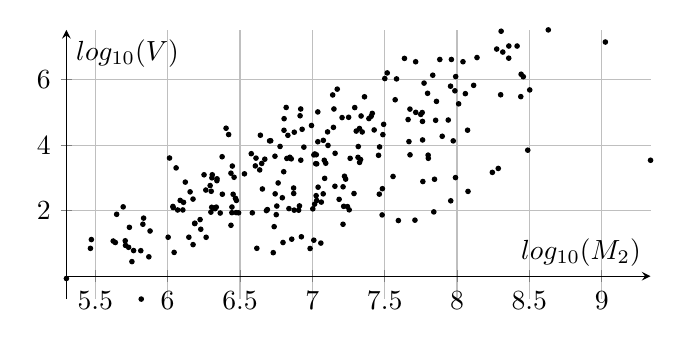
\begin{tikzpicture}
\begin{axis}[width=9cm,height=5cm,
axis lines=middle, xlabel={$log_{10}(M_2)$}, ylabel={$log_{10}(V)$},
xmin=5.300262788643882, xmax=9.337817607630692,
ymin=-0.6989700043360187, ymax=7.518906770153717,
extra tick style={major grid style=black},grid=major]
\addplot [mark=*, only marks, mark size=0.8pt] coordinates {
(5.647511087650302,1.8893017025063101)
(5.692582562274909,2.1161648123118737)
(7.457776654581765,3.690196080028514)
(6.924266515548286,1.2024201977780304)
(7.216770668394846,2.132259689531044)
(6.736250491039094,1.5114377022035417)
(6.263900824669455,2.6290590146121775)
(7.772166756265352,5.894521592313384)
(6.293769252845786,2.766366366191725)
(6.08679853123444,2.313041477993241)
(7.085378962615548,2.986221321921366)
(8.073052438629489,4.456556889858923)
(5.833765270373452,1.7723217067229198)
(6.6106728298275454,3.603570810833047)
(6.30597012059405,3.0024017071695166)
(8.01135938525084,5.261700987694412)
(6.941504326842757,3.9397355140239028)
(6.403689023195856,4.516641125276831)
(7.55794281772462,3.043885997687633)
(7.801742259114062,3.598681098907163)
(7.832429033496079,6.135328024033434)
(7.51781901311406,6.205079897573985)
(6.228963139350912,1.4326486600131065)
(5.8287062875333175,1.5861651813773168)
(6.911021863841136,2.1455071714096623)
(7.254826158872854,2.0255984179691437)
(6.530798713780083,3.1246296093882875)
(8.274468088036434,6.933645525949034)
(7.897747736931188,4.270899536716091)
(6.844839806207417,3.62935862258034)
(6.3274051204258495,2.060225524394167)
(8.316481146610343,6.842255669870494)
(6.175373791317805,2.353723937588949)
(6.854293468338267,3.5823056337991357)
(7.010764072843986,3.7015679850559273)
(7.21217076517489,1.5846542400042958)
(6.444402394827787,2.110910222862586)
(7.03795995395443,4.104214833202107)
(6.187963813507848,1.6174663223227894)
(7.1083857895436475,3.991060867336677)
(7.714825821265492,5.0012477132165465)
(6.8752895843553175,4.3953798183655985)
(8.304971800095547,7.4785919782652845)
(6.636303507733764,3.2433253064048313)
(7.317572660067466,3.957451640973415)
(6.104904475285803,2.021348352175276)
(7.325796058101266,4.508943616417986)
(7.105349074215121,4.404937193444941)
(6.804120410229532,4.453807410461225)
(6.473222079150062,1.9413544870741446)
(5.62369782965714,1.0725506672154261)
(7.250997352029089,4.850314498869368)
(6.459224316888177,3.0197451611626906)
(7.315625731419164,3.6285539698935225)
(7.427477475053893,4.46364463341919)
(7.026496206959709,2.4576490310602934)
(6.6060832766200726,3.3661253696265216)
(7.18526888548742,2.3463529744506384)
(6.421684856027839,4.324195541965875)
(6.335904402636946,2.10744390151416)
(7.582014644162053,6.02280213455429)
(6.437615498426593,1.5531981666918748)
(6.363392521136581,1.9276674643013594)
(6.34035129678636,2.9149510611278813)
(7.762010151213755,4.158550947069742)
(7.667803422511902,4.108868594335923)
(7.326540074714177,3.473347917960341)
(6.919738084515799,5.1043407000326795)
(6.682555250271293,2.0012553521371235)
(8.358266231992452,7.026345332117251)
(7.956847502898422,2.301029995663981)
(6.468604728705185,2.3781070625097422)
(6.038266781443436,2.094988884153331)
(5.8142435991385435,0.7781512503836435)
(6.251518012511634,3.0950995796456136)
(6.802167821086165,3.1888972496655783)
(8.30184972110206,5.538261383647847)
(7.675242757355436,3.7043333313349556)
(8.458299732102924,6.0899937855546495)
(7.939454517948911,4.766828386772239)
(6.804986468601834,4.807671991878399)
(7.636810809124664,6.648699032636881)
(7.881086683344374,6.61545105201613)
(6.819254177642263,5.150568494793861)
(7.390924196641542,4.8112124638026295)
(8.285197877262975,3.288966121430523)
(7.961175323027738,6.615811349712656)
(5.466296585118939,0.8495071588315756)
(6.874497530873762,2.0160241898425677)
(6.6502204611943885,3.4416390361140126)
(6.0362942639242805,2.1285204277315373)
(7.230424676850775,2.962759882966592)
(7.062131249788388,2.26150077319828)
(5.817423886822182,-0.6989700043360187)
(7.1574214368258895,3.7516126536562173)
(6.012874749500376,3.6070754167873944)
(6.447034394923102,3.361809651907951)
(5.764718474842184,0.7820462939763456)
(7.572658071914742,5.385552504732252)
(7.6746820790126336,5.1009217642820515)
(7.839560278999556,1.9619979741284004)
(6.920281564391052,3.5410172928456563)
(6.830978076089829,4.299841039569371)
(6.984383724905092,0.8450980400142567)
(7.594686168986868,1.6983905586147934)
(7.023330954869164,3.434283999039787)
(5.75304426092567,0.4447181689885548)
(6.741791612866611,3.662411516877962)
(6.186993042810472,1.6055205234374688)
(6.9294377787949335,4.484465931154977)
(6.452524568899601,2.4999209514943916)
(7.140766405956862,5.53258298931776)
(7.303517014215802,4.4295863158722355)
(7.989583204791942,3.0093528203388042)
(7.759497575432197,4.995030190801473)
(7.985455216510193,5.6591937624128725)
(7.709384558883058,1.7101173651118162)
(8.115131995079782,5.826252697358896)
(6.994177997738788,4.6003901802505185)
(6.155107289299944,2.5740922170633866)
(7.336993487863417,4.890209444341324)
(7.500784432642139,6.033105739540872)
(6.8240192331184675,3.5942733022270197)
(7.075231819351746,2.513550520346337)
(6.7299284276041655,0.7174534096681198)
(6.8713167196346445,2.5255306856799953)
(7.015821806784398,2.200224938768488)
(7.761494221676318,4.724916108623423)
(8.631002097352543,7.518906770153717)
(8.443188590745871,6.165561437169954)
(6.341315200865003,2.9721756022004318)
(7.974003266097732,4.130724228165944)
(8.415343576497788,7.025922150535285)
(6.265868299473298,1.187520720836463)
(7.261369228169512,3.5977682933213706)
(7.74937309508104,4.938002817389457)
(7.172214636170962,5.710334473753581)
(6.87078272340907,2.691544559996647)
(5.300262788643882,-0.07058107428570727)
(6.654870280891531,2.6621416653736167)
(7.844649063937476,2.9588197569614003)
(9.337817607630692,3.5387155892481412)
(6.689416309290988,2.0328319929325596)
(6.704494726141922,4.130709994038458)
(6.308426740665571,3.0954770343927818)
(6.671462029133507,3.5716942774601916)
(6.7545023758861475,2.140972339302524)
(8.50266545629637,5.686215711535072)
(8.057743581675043,5.57203525029253)
(9.025496341512497,7.148177996370741)
(6.376466544635199,3.6462185097533273)
(7.027448729784829,3.7078425891424036)
(7.058905799011861,1.0104027602969754)
(7.406486341612334,4.880803796054198)
(6.377999766664029,2.5019923596491322)
(7.464750328982202,3.945860088342011)
(8.041238076442523,6.546939748123799)
(7.288091983401679,2.5234342867464368)
(6.743096831936902,2.5131815933913293)
(7.145936779915382,4.542896746285134)
(7.484405922395583,2.6705440298657708)
(6.069144704654302,2.020692678682028)
(7.7966660873049625,5.58324163433773)
(7.003307209436519,2.054883306283622)
(7.414326084467295,4.969853048925632)
(6.750677451375395,1.877946951629188)
(7.212506840030667,2.728353782021228)
(7.360615335985346,5.476289871258936)
(6.6408407489646795,4.3025985161739335)
(6.857624401030012,1.1298988216695378)
(6.915411549923649,4.897401639443342)
(7.242796389648249,2.1242433089466486)
(6.443939333914424,1.9390197764486663)
(5.735553392193666,1.4913616938342726)
(7.222398565686014,3.0505437913005267)
(7.030321652115488,3.4286507867872538)
(6.763654217033682,2.8459932798852767)
(6.792597860384574,2.394951732105887)
(6.905389935573879,2.0141438111386196)
(5.708780255462843,0.9395192526186184)
(7.030208924004791,2.3105547887740983)
(6.4903262792861804,1.9349791314294458)
(5.638301521297118,1.0280287237359604)
(7.293176884526661,5.146962281374943)
(7.076061350348882,4.146913191718257)
(6.616459549203057,0.8512583487190752)
(7.15623928042319,2.744727494900168)
(6.224148579398108,1.7278331076343305)
(6.712339019473114,4.133830565731892)
(6.044794853066763,0.7257631810724322)
(6.577999902780046,3.739466856356103)
(7.955393835994941,5.800150006002939)
(7.333627141970388,3.5599963460325896)
(7.082577289830291,3.5386545102378473)
(5.7300527265942955,0.881691842553922)
(7.487708666654527,4.321050058646378)
(7.800370301408723,3.69469731223624)
(5.870121697786239,0.5906804451232659)
(8.076066245842918,2.588247341812548)
(6.47502245779757,2.3120715213029315)
(6.776950214594808,3.960485047655226)
(5.472753524765399,1.1179739564353584)
(6.301135082213642,2.59193522773433)
(7.714217071699241,6.5461988792249155)
(7.010344104840682,1.0988359341978273)
(6.1096453563010105,2.254427221540668)
(6.146625018391679,1.189056236092315)
(7.764005886984079,2.8893311951884435)
(7.039758047307564,2.717080782383067)
(6.298960218263159,1.9551754732533502)
(6.175587474902988,0.9631973520922511)
(6.437442326282366,3.1436587344094393)
(6.838347348242559,2.062525008876046)
(5.706793713240614,1.0804274291099996)
(5.878410909871675,1.3795644887491045)
(6.304505822597521,2.103251815334661)
(8.48907599373849,3.846428754772363)
(6.058438172384501,3.305474207654434)
(6.797287142515685,1.0280287237359604)
(8.138183053298057,6.6743104750179905)
(7.344702241442134,4.402329459586968)
(7.8580787087941655,5.336247054846863)
(7.662081722840741,4.781308249662078)
(8.357610751942017,6.655799142923314)
(7.991000786832456,6.093707734963201)
(7.205530612054983,4.8417115785119)
(7.149378848203527,5.104286217017372)
(7.016882813474166,3.7308460003706565)
(6.1219794922001,2.871602121022312)
(8.440771127599923,5.48085802900349)
(6.585223889845297,1.9343498983389538)
(7.037747876448219,5.014215921798604)
(6.003347204379362,1.1889738194896236)
(8.244260181749404,3.1688179992656647)
(7.852282308064531,4.758705288570067)
(7.493122782909744,4.635883859129601)
(7.092757547623055,3.448517380461247)
(7.462936697988623,2.5037437348381983)
(7.482397355847451,1.8698490538656023)
};
\end{axis}\end{tikzpicture}

  \caption{The relationship between the size of the Git repository in bytes and its Volatility ($Z$ is set to 64)}
  \label{fig:2}
\end{figure}

The Figure~\ref{fig:1} demonstrates the same relationship as the Figure~\ref{fig:1},
but the parameter of the Volatility formula is set to 32 instead of 64. The
trend of the graph didn't change much.

\begin{figure}[h]
  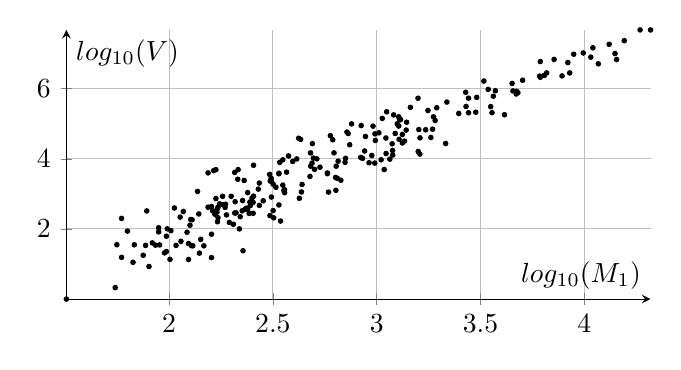
\begin{tikzpicture}
\begin{axis}[width=9cm,height=5cm,
axis lines=middle, xlabel={$log_{10}(M_1)$}, ylabel={$log_{10}(V)$},
xmin=1.5051499783199058, xmax=4.319480828050337,
ymin=0.0, ymax=7.6772370457911805,
extra tick style={major grid style=black},grid=major]
\addplot [mark=*, only marks, mark size=0.8pt] coordinates {
(2.110589710299249,2.262302739777867)
(2.02530586526477,2.5973294642385873)
(2.2253092817258624,3.690196080028514)
(1.919078092376074,1.6028943710260306)
(2.3783979009481375,2.558708570533166)
(1.9493900066449126,1.9164539485499248)
(2.5563025007672873,3.1198330248869945)
(3.8930401119571174,6.364558724413771)
(2.827369273053825,3.3891452293866777)
(2.2041199826559246,2.638489256954637)
(2.810232517995084,3.443079228243638)
(2.945960703577568,4.6379942231041476)
(2.53655844257153,2.2242965463637496)
(2.9319661147281724,4.013396099545609)
(2.3304137733491905,3.4164740791002206)
(3.048053173115609,5.341194557583745)
(2.681241237375587,4.16879496467357)
(2.624282095835668,4.586727921309507)
(2.762678563727436,3.5769523529524228)
(2.187520720836463,3.598681098907163)
(3.9301336458411176,6.450164612882969)
(3.8189513116401725,6.450679481517348)
(1.9867717342662448,1.792803538259554)
(2.3096301674258983,2.132697741200264)
(2.187520720836463,2.620136054973757)
(2.0530784434834195,2.3380135619215827)
(2.3617278360175926,3.3829007864087446)
(3.949194774237982,6.983116669885224)
(2.9934362304976116,4.5256774220994425)
(2.850033257689769,4.0130427280764644)
(2.2095150145426303,2.519040038648344)
(3.9951962915971793,7.019357942369708)
(2.4533183400470375,2.803581252987421)
(3.077367905284156,4.1076066132455225)
(2.4065401804339546,3.8165285244959515)
(2.086359830674748,1.9055883322161145)
(2.2329961103921536,2.5796077332934737)
(3.208710019906401,4.5972622293668834)
(1.7993405494535815,1.9386864728992093)
(3.1338581252033344,4.504487853338962)
(3.4426365257822313,5.313885666951742)
(3.2692793897718984,4.844570103165263)
(4.2689989585426735,7.6772370457911805)
(2.5289167002776547,3.587952604113285)
(3.332236415491443,4.436585455266805)
(2.2304489213782737,2.4780050288276705)
(3.2030328870147105,4.834739729183914)
(3.010723865391773,4.741301986356266)
(2.633468455579586,4.553081633070497)
(2.4857214264815797,2.381154335418895)
(1.9542425094393248,1.5440680443502754)
(3.2736955879300917,5.1966350380670265)
(3.0362295440862943,3.694904431295289)
(2.5327543789924976,3.8987129958271343)
(2.8627275283179743,4.721991876784904)
(2.3541084391474008,2.810712454478117)
(2.804820678721162,3.7890386190730334)
(2.2430380486862944,2.7169766308620673)
(2.7767011839884104,4.659959912412958)
(2.4345689040341987,2.6719951757086022)
(3.5162708827293403,6.21802602640967)
(2.3384564936046046,2.00225999372902)
(2.404833716619938,2.445669057229761)
(2.487138375477186,3.3665235266024083)
(2.869818207979328,4.40197232995542)
(3.261024833992397,4.6077587444024175)
(3.021189299069938,3.9716357556754476)
(3.2469906992415494,5.378567587896862)
(2.3521825181113623,2.5172486965011185)
(4.120014252078067,7.266239774939123)
(1.7708520116421442,2.301029995663981)
(2.3180633349627615,2.7765195847878124)
(2.3729120029701067,2.59381054213724)
(1.8750612633916997,1.2486419262711075)
(2.5289167002776547,3.574199688683068)
(2.700703717145019,3.6990405714559045)
(3.442322955745574,5.729495835129515)
(2.81424759573192,3.933035114388899)
(3.703033304733686,6.241576113211356)
(3.1442627737619904,5.043308460264328)
(2.925312091499649,4.9493233121091995)
(3.7884512070234555,6.774495841715148)
(3.854731017213942,6.83429923684893)
(3.162265614298021,5.468074850726045)
(3.1149444157125843,5.118935293622146)
(2.726727209026572,3.7612643543349478)
(4.031650793551264,6.899189962387286)
(1.7708520116421442,1.1903316981702914)
(2.3159703454569174,2.4541224404106807)
(3.0633333589517493,3.9909028196432557)
(2.2355284469075487,2.622119785257873)
(2.8020892578817325,3.4689083009620356)
(2.404833716619938,2.75815462196739)
(1.5051499783199058,0.0)
(2.6148972160331345,3.996852047402435)
(2.7118072290411908,4.000106586473919)
(2.963315511386111,3.888868748898837)
(2.093421685162235,1.1296338578306893)
(3.3382572302462554,5.618702315721097)
(3.5493711523331766,5.488696514387222)
(2.3856062735983117,2.443028170214854)
(2.923244018630276,4.039051840495479)
(3.123851640967086,4.6933511988637076)
(1.9867717342662448,1.3547148546772567)
(2.008600171761917,1.9524842298006044)
(2.847572659142112,3.8995170765170237)
(2.2041199826559246,1.1835334518952294)
(3.20002926655377,4.207195156637595)
(2.1003705451175625,2.1058106306219035)
(2.8567288903828825,4.762786061433896)
(2.803457115648414,3.1019848770322884)
(3.4820155764507117,5.7518175680022035)
(2.9916690073799486,4.711947322362851)
(2.678518379040114,3.4986834570687377)
(3.106190897263415,5.196452887039194)
(3.6737579365495763,5.925733474318332)
(2.2329961103921536,2.2061509815962594)
(3.6526330680831096,6.150780044302783)
(3.098989639401177,4.998758073939888)
(2.2988530764097064,2.9298870301462947)
(3.4772659954248524,5.328533952986147)
(3.785756799962643,6.359799301782963)
(2.976349979003273,4.0939481814479315)
(1.8920946026904801,2.513550520346337)
(1.9777236052888476,1.3174204118682353)
(2.2253092817258624,2.866976148876714)
(2.0681858617461617,2.497850739583007)
(3.106190897263415,4.934361744799739)
(4.319480828050337,7.675700860383867)
(3.788663213120857,6.325038775750639)
(2.4913616938342726,3.446198139358112)
(3.1078880251827985,4.555587471241042)
(4.04166896647561,7.166295410492781)
(1.7481880270062005,1.550228353055094)
(2.214843848047698,3.6650178254124723)
(3.026941627959029,5.1528028721313035)
(3.6565772913961134,5.9362359084554255)
(2.2576785748691846,2.93091266266495)
(1.7403626894942439,0.325853579630288)
(2.4297522800024076,3.136185294406502)
(2.5477747053878224,3.2508050720687187)
(2.6821450763738315,3.790291867608943)
(2.501059262217751,2.5234987232333586)
(2.6901960800285134,4.432571138693195)
(2.5658478186735176,3.6196529213180586)
(2.695481676490197,4.020510442157546)
(2.2695129442179165,2.613237585979202)
(3.5373152731120094,5.980735279686611)
(3.428782511496954,5.896533067257859)
(4.192957529884656,7.370131341850384)
(2.5477747053878224,3.9703391264377035)
(2.575187844927661,4.082928915015129)
(2.093421685162235,1.5839197657622832)
(3.3955011243056257,5.292302991394904)
(2.4065401804339546,2.9357758877471096)
(2.7944880466591693,4.169245562689372)
(3.920957705955449,6.745908417263599)
(2.5563025007672873,3.034503122728775)
(2.6374897295125104,3.0553435753045908)
(3.236033147117636,4.8280795905567455)
(2.5526682161121927,3.0978162597302563)
(2.3654879848908994,2.5585674054136884)
(3.1992064791616572,5.72745178640297)
(2.143014800254095,2.4274590595134673)
(3.11092624226642,5.117424432051345)
(2.2355284469075487,2.3204232596351417)
(2.7678976160180904,3.051125898213724)
(3.680335513414563,5.886350543877396)
(2.7881683711411673,4.544587114776956)
(2.3560258571931225,1.3778445084799629)
(2.8790958795000723,4.9960725588873185)
(2.390935107103379,2.6676863818028043)
(1.9912260756924949,2.002038944995054)
(1.9493900066449126,2.03462845662532)
(2.501059262217751,3.276848638899351)
(2.9907826918031377,3.8786103496109385)
(2.1367205671564067,3.07059193151204)
(2.271841606536499,2.7032913781186614)
(2.342422680822206,2.3491695611487784)
(2.1673173347481756,1.5185139398778873)
(2.2600713879850747,2.689935320797475)
(2.220108088040055,2.4194836892167357)
(1.8325089127062362,1.5481846105041364)
(3.2893659515200313,5.456964370119124)
(3.123851640967086,4.4525897179307865)
(2.0043213737826426,1.1332485074731735)
(2.6404814369704215,3.267875419318897)
(2.503790683057181,2.3162699622147276)
(3.0445397603924107,4.592909958815318)
(1.8260748027008262,1.0487330483239683)
(2.9420080530223127,4.223384879824185)
(3.571825249040829,5.941946077436817)
(2.6884198220027105,3.877385745315471)
(2.5954962218255737,3.9252927489750093)
(2.1461280356782377,1.3094450067437902)
(3.0891983668051486,4.723499797068384)
(3.045322978786657,4.151669572697138)
(1.9030899869919433,0.9282007077701632)
(2.3996737214810375,2.8841224508556467)
(2.6273658565927325,2.8740782685867816)
(3.074450718954591,4.427744888371816)
(2.107209969647868,1.525353364358841)
(2.3783979009481375,3.0358583888013415)
(4.06774020292624,6.7096949219196516)
(2.1139433523068365,1.5185139398778873)
(2.3891660843645326,2.7678358518902)
(1.9344984512435675,1.5367069447558732)
(2.4345689040341987,3.3084576941893036)
(2.514547752660286,3.1881371786857495)
(2.276461804173244,2.4000854921437007)
(1.8864907251724818,1.5303161466621058)
(2.484299839346786,3.55612699279135)
(2.322219294733919,2.4602533294302167)
(2.0569048513364723,1.6465584905107151)
(2.2041199826559246,1.848873045443868)
(2.5289167002776547,2.6842782740987046)
(3.2081725266671213,4.135119550289691)
(2.332438459915605,3.691788524402698)
(2.0334237554869494,1.5298793038824618)
(4.148263229636878,7.0035329745442585)
(3.1420764610732843,4.820796891979662)
(3.672467313068082,5.849008472274008)
(3.555457217204649,5.315790731553568)
(4.156094630639427,6.832396312284101)
(3.807805532270624,6.37868473130767)
(3.6158448828747014,5.257704341757222)
(3.430558769522757,5.492966269350169)
(3.0766404436703416,4.23865501199016)
(2.492760389026837,3.3676354197905107)
(3.562054829656378,5.786084981034844)
(2.290034611362518,2.184562387724883)
(3.081707270097349,5.2531153885146376)
(2.1522883443830563,1.702430536445525)
(2.762678563727436,3.5952706989087084)
(3.2817149700272954,5.092761511345405)
(2.982271233039568,4.932645506069353)
(2.3159703454569174,3.6107488579702385)
(2.492760389026837,2.9100061919974953)
(2.103803720955957,2.268433951164878)
};
\end{axis}\end{tikzpicture}

  \caption{The relationship between the number of files in the repository and its Volatility ($Z$ is set to 32)}
  \label{fig:3}
\end{figure}

The Figure~\ref{fig:1} demonstrates the same relationship as the Figure~\ref{fig:1},
but this time the parameter of the Volatility formula is increased to 128
instead of the original value of 64. The trend of the graph didn't change much.

\begin{figure}[h]
  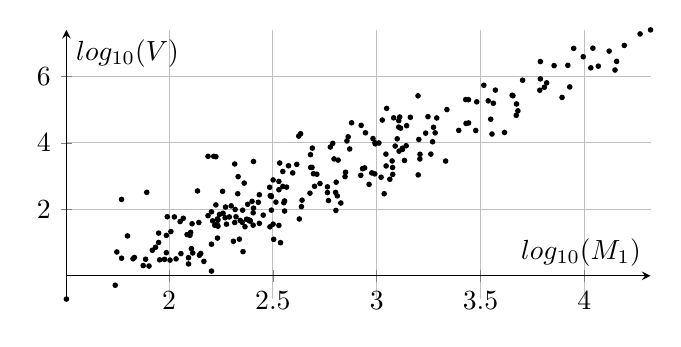
\begin{tikzpicture}
\begin{axis}[width=9cm,height=5cm,
axis lines=middle, xlabel={$log_{10}(M_1)$}, ylabel={$log_{10}(V)$},
xmin=1.5051499783199058, xmax=4.319480828050337,
ymin=-0.6989700043360187, ymax=7.40283643530911,
extra tick style={major grid style=black},grid=major]
\addplot [mark=*, only marks, mark size=0.8pt] coordinates {
(2.110589710299249,1.5669422901437675)
(2.02530586526477,1.7729500567292305)
(2.2253092817258624,3.585122186306815)
(1.919078092376074,0.7690078709437738)
(2.3783979009481375,1.6958706549653662)
(1.9493900066449126,1.28596624926898)
(2.5563025007672873,2.2543727070425024)
(3.8930401119571174,5.3694088342993)
(2.827369273053825,2.191988917371768)
(2.2041199826559246,1.926195402607449)
(2.810232517995084,2.407088295369347)
(2.945960703577568,4.305503990686615)
(2.53655844257153,0.9980214338196041)
(2.9319661147281724,3.2246337619020538)
(2.3304137733491905,2.4716776477004294)
(3.048053173115609,5.040265567625035)
(2.681241237375587,3.6468330001022595)
(2.624282095835668,4.205156978860487)
(2.762678563727436,2.5064627508995176)
(2.187520720836463,3.598681098907163)
(3.9301336458411176,5.685832988965562)
(3.8189513116401725,5.809171898837439)
(1.9867717342662448,1.217483944213906)
(2.3096301674258983,1.0399279467825742)
(2.187520720836463,1.8095597146352675)
(2.0530784434834195,1.634843531641697)
(2.3617278360175926,2.7918144443042223)
(3.949194774237982,6.846276331395443)
(2.9934362304976116,3.9742222792312676)
(2.850033257689769,3.1177231366683396)
(2.2095150145426303,1.6564176536186217)
(3.9951962915971793,6.595782932085179)
(2.4533183400470375,1.827418045527655)
(3.077367905284156,3.0532422259807155)
(2.4065401804339546,3.4426051789648007)
(2.086359830674748,1.2413579905076735)
(2.2329961103921536,1.7124867699010977)
(3.208710019906401,3.6582297427843082)
(1.7993405494535815,1.2020269930661591)
(3.1338581252033344,3.4737479736288965)
(3.4426365257822313,4.601747428126263)
(3.2692793897718984,4.036549807763436)
(4.2689989585426735,7.2803724732676764)
(2.5289167002776547,2.8416606696585505)
(3.332236415491443,3.454832570800259)
(2.2304489213782737,1.5604100819240836)
(3.2030328870147105,4.105464329236351)
(3.010723865391773,3.998600767776147)
(2.633468455579586,4.277998644200288)
(2.4857214264815797,1.47416685910302)
(1.9542425094393248,0.4817661591186044)
(3.2736955879300917,4.470728915640691)
(3.0362295440862943,2.4713375589852835)
(2.5327543789924976,3.3953846446256795)
(2.8627275283179743,4.18340509467196)
(2.3541084391474008,1.9761305930095365)
(2.804820678721162,2.8191782138483577)
(2.2430380486862944,1.8516659456552422)
(2.7767011839884104,3.877336785252073)
(2.4345689040341987,1.578788648934896)
(3.5162708827293403,5.735807092518518)
(2.3384564936046046,1.1034498206919512)
(2.404833716619938,1.5257920876902649)
(2.487138375477186,2.411002052572627)
(2.869818207979328,3.8180824858479245)
(3.261024833992397,3.6641794399488545)
(3.021189299069938,2.9671932937405185)
(3.2469906992415494,4.7916807094796)
(2.3521825181113623,1.6096131292614633)
(4.120014252078067,6.7646484514266545)
(1.7708520116421442,2.301029995663981)
(2.3180633349627615,1.9975431977341054)
(2.3729120029701067,1.7025908222767465)
(1.8750612633916997,0.3099848390259598)
(2.5289167002776547,2.5917726685297207)
(2.700703717145019,2.694793164516775)
(3.442322955745574,5.301628908893861)
(2.81424759573192,3.484193945480137)
(3.703033304733686,5.888145847649928)
(3.1442627737619904,4.5190049852174)
(2.925312091499649,4.529474686915843)
(3.7884512070234555,6.450063366412974)
(3.854731017213942,6.327636768418774)
(3.162265614298021,4.7721806058146035)
(3.1149444157125843,4.444961980375294)
(2.726727209026572,2.7780941026119197)
(4.031650793551264,6.261115540636362)
(1.7708520116421442,0.5300573300498526)
(2.3159703454569174,1.6050302631210351)
(3.0633333589517493,2.90687353472207)
(2.2355284469075487,1.682686478249768)
(2.8020892578817325,2.511510792335396)
(2.404833716619938,1.8976270912904412)
(1.5051499783199058,-0.6989700043360187)
(2.6148972160331345,3.3553002524700486)
(2.7118072290411908,3.057991946978772)
(2.963315511386111,2.7530672083988135)
(2.093421685162235,0.3590219434559701)
(3.3382572302462554,5.0049464633851555)
(3.5493711523331766,4.714038135995996)
(2.3856062735983117,1.6653724963243357)
(2.923244018630276,3.0240682516066295)
(3.123851640967086,3.805172993507661)
(1.9867717342662448,0.6968463110467863)
(2.008600171761917,1.333355660943502)
(2.847572659142112,2.9861909602028067)
(2.2041199826559246,0.1428930526344926)
(3.20002926655377,3.037914447262529)
(2.1003705451175625,1.217483944213906)
(2.8567288903828825,4.060229304960798)
(2.803457115648414,1.9680468786234884)
(3.4820155764507117,5.237853674666972)
(2.9916690073799486,4.004715868114394)
(2.678518379040114,2.4891546023219853)
(3.106190897263415,4.671604036124467)
(3.6737579365495763,5.173005284388308)
(2.2329961103921536,1.136864635509919)
(3.6526330680831096,5.43559539859391)
(3.098989639401177,4.124291384179315)
(2.2988530764097064,2.10646713223443)
(3.4772659954248524,4.374788165083977)
(3.785756799962643,5.586448854634285)
(2.976349979003273,3.0981301126817042)
(1.8920946026904801,2.513550520346337)
(1.9777236052888476,0.4973246404131362)
(2.2253092817258624,2.1344321248958393)
(2.0681858617461617,1.7323937598229684)
(3.106190897263415,4.4763398204270946)
(4.319480828050337,7.40283643530911)
(3.788663213120857,5.92764709519543)
(2.4913616938342726,2.4098767909570706)
(3.1078880251827985,3.753144155892327)
(4.04166896647561,6.8518041238140395)
(1.7481880270062005,0.7185655603355326)
(2.214843848047698,3.5977682933213706)
(3.026941627959029,4.689010022444967)
(3.6565772913961134,5.4205041027724015)
(2.2576785748691846,2.5435542889927105)
(1.7403626894942439,-0.28254659033188007)
(2.4297522800024076,2.21409842012804)
(2.5477747053878224,2.6891138604711378)
(2.6821450763738315,3.26324351273289)
(2.501059262217751,1.556101391910356)
(2.6901960800285134,3.8432902903891395)
(2.5658478186735176,2.6704446603438896)
(2.695481676490197,3.073168262265101)
(2.2695129442179165,1.7477315955545731)
(3.5373152731120094,5.266878280969938)
(3.428782511496954,5.30437697188792)
(4.192957529884656,6.93600781287549)
(2.5477747053878224,3.1403705365859675)
(2.575187844927661,3.3127325681624282)
(2.093421685162235,0.545444573041644)
(3.3955011243056257,4.3782663206806225)
(2.4065401804339546,2.0383913291679225)
(2.7944880466591693,3.5182761378249783)
(3.920957705955449,6.3354135161331495)
(2.5563025007672873,1.9506661500143827)
(2.6374897295125104,2.0817586689200165)
(3.236033147117636,4.295154337206611)
(2.5526682161121927,2.2012149920034085)
(2.3654879848908994,1.478233405133459)
(3.1992064791616572,5.417177219790012)
(2.143014800254095,1.6048657799352977)
(3.11092624226642,4.779972909013159)
(2.2355284469075487,1.4943802602138099)
(2.7678976160180904,2.266905888060436)
(3.680335513414563,4.965162609505758)
(2.7881683711411673,3.9870008043466676)
(2.3560258571931225,0.7286918862260852)
(2.8790958795000723,4.606689930116752)
(2.390935107103379,1.6467303862147695)
(1.9912260756924949,1.778687085686697)
(1.9493900066449126,1.0045476278411987)
(2.501059262217751,2.8868819089317563)
(2.9907826918031377,3.069042417426944)
(2.1367205671564067,2.555094448578319)
(2.271841606536499,2.070934570163774)
(2.342422680822206,1.6671547761307868)
(2.1673173347481756,0.4354446247810428)
(2.2600713879850747,1.8836614351536174)
(2.220108088040055,1.5209745384255442)
(1.8325089127062362,0.5537553119450078)
(3.2893659515200313,4.752136066539505)
(3.123851640967086,3.8417537004204894)
(2.0043213737826426,0.47339338156395316)
(2.6404814369704215,2.2774309272617255)
(2.503790683057181,1.0986193551569496)
(3.0445397603924107,3.663789045620996)
(1.8260748027008262,0.5131189080898846)
(2.9420080530223127,3.250590191514692)
(3.571825249040829,5.590440748821799)
(2.6884198220027105,3.262143861876735)
(2.5954962218255737,3.098146933280924)
(2.1461280356782377,0.6201164040057162)
(3.0891983668051486,3.906515584098993)
(3.045322978786657,3.307580308408328)
(1.9030899869919433,0.29512113539904455)
(2.3996737214810375,2.241963560482206)
(2.6273658565927325,1.711103918013772)
(3.074450718954591,3.4576153564437657)
(2.107209969647868,0.818079197430316)
(2.3783979009481375,2.1535690140832493)
(4.06774020292624,6.311103423764814)
(2.1139433523068365,0.6888303725747819)
(2.3891660843645326,1.670191262631623)
(1.9344984512435675,0.8598212968142824)
(2.4345689040341987,2.4409673570759245)
(2.514547752660286,2.2185792650602605)
(2.276461804173244,1.5549294535661138)
(1.8864907251724818,0.4996870826184038)
(2.484299839346786,2.6651321499665603)
(2.322219294733919,1.7780196260379353)
(2.0569048513364723,0.6690067812687859)
(2.2041199826559246,0.9520925325812964)
(2.5289167002776547,1.517075877353566)
(3.2081725266671213,3.5184515964825955)
(2.332438459915605,2.9866903218604275)
(2.0334237554869494,0.5093059379876602)
(4.148263229636878,6.195191851298916)
(3.1420764610732843,3.9150933697870274)
(3.672467313068082,4.830983257679388)
(3.555457217204649,4.268297987785405)
(4.156094630639427,6.453985894324515)
(3.807805532270624,5.67565465877563)
(3.6158448828747014,4.315701179982193)
(3.430558769522757,4.588189005058379)
(3.0766404436703416,3.2609295835299243)
(2.492760389026837,2.387199081371098)
(3.562054829656378,5.194296738484303)
(2.290034611362518,1.772048651413861)
(3.081707270097349,4.756190461627315)
(2.1522883443830563,0.6716959191074446)
(2.762678563727436,2.678046629207955)
(3.2817149700272954,4.303413479025716)
(2.982271233039568,4.131230384240135)
(2.3159703454569174,3.3668642444498134)
(2.492760389026837,1.9772568728446285)
(2.103803720955957,1.3093553843587795)
};
\end{axis}\end{tikzpicture}

  \caption{The relationship between the number of files in the repository and its Volatility ($Z$ is set to 128)}
  \label{fig:4}
\end{figure}

\section{Discussion}
\label{sec:discussion}

It was demonstrated that the size of the source code is an important
factor negatively affecting maintainability and other quality characteristicts.
For example, \citet{heitlager2007} suggested to consider ``volume''
(the number of lines per file, the number of methods in a class,
and so on) as a primary contributor to an aggregate maintainability index
of a software because ``it is fairly intuitive that the total size of a system should
feature heavily in any measure of maintainability.''

However, the discussion of whether larger repositories are a better
practice than smaller ones is still open. Google, for example, advocates
for larger ones, known as ``monolithic,'' which tend to keep many modules
and components in one Git space, simplifying dependencies management~\citep{jaspan2018}.
As was demonstrated in our research, larger repositories will tend to
have maintenance anomalies: some parts of source code will be changed much
less frequently than other parts. Moreover, the distance between ``popular''
parts and ``abandoned'' ones will grow when the size of the repository grows.

These maintenance anomalies will lead to maintability and quality problems
mostly because it will be difficult for programmers to quickly switch between
different contexts inside one repository: one set of files is being modified
every day, while another one stays untouched for months. A programmer will
try to avoid making changes to the part that is abandonded because it won't
look like code that is expecting changes.

Also, maintenance anomalies is a sign of differences in customer demand
for the source code components. The module with smaller frequency of changes
must be released less frequently than the module that is being edited every day.
Not paying attention to the growing Volatility of the repository means
ignoring anomalies and, because of that, redundant releasing of the code
that doesn't require new releases. Moreover, releasing larger software modules
usually means longer build cycles, which are the key failure factor of
continuous delivery, as explained by~\cite{humble2010}. Getting rid of
maintenance anomalies may help reduce build cycles.

It would be beneficial in future researches to analyze the relationship between
Volatility and other parameters of source code repositories,
such as
the programming language being used,
the popularity in GitHub (the number of stars and forks),
the total number of lines of code,
the average number of lines of code per file,
the number of Git commit authors,
the total age of the repository,
the number of issues and pull requests in GitHub,
and many others.
Would be interesting to empiricially demonstrate which of these parameters
(or combinations of them)
impact the behavior of Volatility and in which direction.

\section{Conclusion}
\label{sec:conclusion}

A new source code Volatility metric was introduced and applied
to \thetotalrepos{} open source Java repositories from GitHub. It was
empirically demonstrated that larger repositories have higher values
of the Volatility metric.

The source code of Ruby and Python scripts used to do the research
is available in GitHub repository:\newline\texttt{yegor256/volatility-vs-size}.

\bibliographystyle{ACM-Reference-Format}
\bibliography{main}
\clearpage

\end{document}
